\documentclass[twoside]{book}

% Packages required by doxygen
\usepackage{fixltx2e}
\usepackage{calc}
\usepackage{doxygen}
\usepackage[export]{adjustbox} % also loads graphicx
\usepackage{graphicx}
\usepackage[utf8]{inputenc}
\usepackage{makeidx}
\usepackage{multicol}
\usepackage{multirow}
\PassOptionsToPackage{warn}{textcomp}
\usepackage{textcomp}
\usepackage[nointegrals]{wasysym}
\usepackage[table]{xcolor}

% Font selection
\usepackage[T1]{fontenc}
\usepackage[scaled=.90]{helvet}
\usepackage{courier}
\usepackage{amssymb}
\usepackage{sectsty}
\renewcommand{\familydefault}{\sfdefault}
\allsectionsfont{%
  \fontseries{bc}\selectfont%
  \color{darkgray}%
}
\renewcommand{\DoxyLabelFont}{%
  \fontseries{bc}\selectfont%
  \color{darkgray}%
}
\newcommand{\+}{\discretionary{\mbox{\scriptsize$\hookleftarrow$}}{}{}}

% Page & text layout
\usepackage{geometry}
\geometry{%
  a4paper,%
  top=2.5cm,%
  bottom=2.5cm,%
  left=2.5cm,%
  right=2.5cm%
}
\tolerance=750
\hfuzz=15pt
\hbadness=750
\setlength{\emergencystretch}{15pt}
\setlength{\parindent}{0cm}
\setlength{\parskip}{0.2cm}
\makeatletter
\renewcommand{\paragraph}{%
  \@startsection{paragraph}{4}{0ex}{-1.0ex}{1.0ex}{%
    \normalfont\normalsize\bfseries\SS@parafont%
  }%
}
\renewcommand{\subparagraph}{%
  \@startsection{subparagraph}{5}{0ex}{-1.0ex}{1.0ex}{%
    \normalfont\normalsize\bfseries\SS@subparafont%
  }%
}
\makeatother

% Headers & footers
\usepackage{fancyhdr}
\pagestyle{fancyplain}
\fancyhead[LE]{\fancyplain{}{\bfseries\thepage}}
\fancyhead[CE]{\fancyplain{}{}}
\fancyhead[RE]{\fancyplain{}{\bfseries\leftmark}}
\fancyhead[LO]{\fancyplain{}{\bfseries\rightmark}}
\fancyhead[CO]{\fancyplain{}{}}
\fancyhead[RO]{\fancyplain{}{\bfseries\thepage}}
\fancyfoot[LE]{\fancyplain{}{}}
\fancyfoot[CE]{\fancyplain{}{}}
\fancyfoot[RE]{\fancyplain{}{\bfseries\scriptsize Generated on Tue Dec 1 2015 01\+:01\+:22 for Ind\+Inf03\+\_\+\+Ampelsteuerung\+\_\+\+Interrupts\+\_\+\+Weinb\+\_\+5\+B\+H\+I\+T by Doxygen }}
\fancyfoot[LO]{\fancyplain{}{\bfseries\scriptsize Generated on Tue Dec 1 2015 01\+:01\+:22 for Ind\+Inf03\+\_\+\+Ampelsteuerung\+\_\+\+Interrupts\+\_\+\+Weinb\+\_\+5\+B\+H\+I\+T by Doxygen }}
\fancyfoot[CO]{\fancyplain{}{}}
\fancyfoot[RO]{\fancyplain{}{}}
\renewcommand{\footrulewidth}{0.4pt}
\renewcommand{\chaptermark}[1]{%
  \markboth{#1}{}%
}
\renewcommand{\sectionmark}[1]{%
  \markright{\thesection\ #1}%
}

% Indices & bibliography
\usepackage{natbib}
\usepackage[titles]{tocloft}
\setcounter{tocdepth}{3}
\setcounter{secnumdepth}{5}
\makeindex

% Hyperlinks (required, but should be loaded last)
\usepackage{ifpdf}
\ifpdf
  \usepackage[pdftex,pagebackref=true]{hyperref}
\else
  \usepackage[ps2pdf,pagebackref=true]{hyperref}
\fi
\hypersetup{%
  colorlinks=true,%
  linkcolor=blue,%
  citecolor=blue,%
  unicode%
}

% Custom commands
\newcommand{\clearemptydoublepage}{%
  \newpage{\pagestyle{empty}\cleardoublepage}%
}


%===== C O N T E N T S =====

\begin{document}

% Titlepage & ToC
\hypersetup{pageanchor=false,
             bookmarks=true,
             bookmarksnumbered=true,
             pdfencoding=unicode
            }
\pagenumbering{roman}
\begin{titlepage}
\vspace*{7cm}
\begin{center}%
{\Large Ind\+Inf03\+\_\+\+Ampelsteuerung\+\_\+\+Interrupts\+\_\+\+Weinb\+\_\+5\+B\+H\+I\+T \\[1ex]\large 1.\+0 }\\
\vspace*{1cm}
{\large Generated by Doxygen 1.8.10}\\
\vspace*{0.5cm}
{\small Tue Dec 1 2015 01:01:22}\\
\end{center}
\end{titlepage}
\clearemptydoublepage
\tableofcontents
\clearemptydoublepage
\pagenumbering{arabic}
\hypersetup{pageanchor=true}

%--- Begin generated contents ---
\chapter{Module Index}
\section{Modules}
Here is a list of all modules\+:\begin{DoxyCompactList}
\item \contentsline{section}{C\+M\+S\+I\+S}{\pageref{group___c_m_s_i_s}}{}
\begin{DoxyCompactList}
\item \contentsline{section}{Stm32f3xx\+\_\+system}{\pageref{group__stm32f3xx__system}}{}
\begin{DoxyCompactList}
\item \contentsline{section}{S\+T\+M32\+F3xx\+\_\+\+System\+\_\+\+Private\+\_\+\+Includes}{\pageref{group___s_t_m32_f3xx___system___private___includes}}{}
\item \contentsline{section}{S\+T\+M32\+F3xx\+\_\+\+System\+\_\+\+Private\+\_\+\+Types\+Definitions}{\pageref{group___s_t_m32_f3xx___system___private___types_definitions}}{}
\item \contentsline{section}{S\+T\+M32\+F3xx\+\_\+\+System\+\_\+\+Private\+\_\+\+Defines}{\pageref{group___s_t_m32_f3xx___system___private___defines}}{}
\item \contentsline{section}{S\+T\+M32\+F3xx\+\_\+\+System\+\_\+\+Private\+\_\+\+Macros}{\pageref{group___s_t_m32_f3xx___system___private___macros}}{}
\item \contentsline{section}{S\+T\+M32\+F3xx\+\_\+\+System\+\_\+\+Private\+\_\+\+Variables}{\pageref{group___s_t_m32_f3xx___system___private___variables}}{}
\item \contentsline{section}{S\+T\+M32\+F3xx\+\_\+\+System\+\_\+\+Private\+\_\+\+Function\+Prototypes}{\pageref{group___s_t_m32_f3xx___system___private___function_prototypes}}{}
\item \contentsline{section}{S\+T\+M32\+F3xx\+\_\+\+System\+\_\+\+Private\+\_\+\+Functions}{\pageref{group___s_t_m32_f3xx___system___private___functions}}{}
\end{DoxyCompactList}
\end{DoxyCompactList}
\end{DoxyCompactList}

\chapter{Data Structure Index}
\section{Data Structures}
Here are the data structures with brief descriptions\+:\begin{DoxyCompactList}
\item\contentsline{section}{\hyperlink{structampelparameter}{ampelparameter} }{\pageref{structampelparameter}}{}
\end{DoxyCompactList}

\chapter{File Index}
\section{File List}
Here is a list of all documented files with brief descriptions\+:\begin{DoxyCompactList}
\item\contentsline{section}{src/\hyperlink{ampel_8h}{ampel.\+h} \\*Definition der States \& Events }{\pageref{ampel_8h}}{}
\item\contentsline{section}{src/\hyperlink{ampelsteuerung_8c}{ampelsteuerung.\+c} \\*Implementierung einer Event Centric State Machine zur Steuerung einer Ampel }{\pageref{ampelsteuerung_8c}}{}
\item\contentsline{section}{src/\hyperlink{control_8c}{control.\+c} \\*Steuern der benoetigten L\+E\+Ds am Board }{\pageref{control_8c}}{}
\item\contentsline{section}{src/\hyperlink{control_8h}{control.\+h} \\*Definition der Funktionen }{\pageref{control_8h}}{}
\item\contentsline{section}{src/\hyperlink{main_8c}{main.\+c} \\*Hauptklasse }{\pageref{main_8c}}{}
\item\contentsline{section}{src/\hyperlink{stm32f3xx__it_8c}{stm32f3xx\+\_\+it.\+c} \\*Default Interrupt Service Routines }{\pageref{stm32f3xx__it_8c}}{}
\item\contentsline{section}{src/\hyperlink{system__stm32f3xx_8c}{system\+\_\+stm32f3xx.\+c} \\*C\+M\+S\+I\+S Cortex-\/\+M4 Device Peripheral Access Layer System Source File }{\pageref{system__stm32f3xx_8c}}{}
\end{DoxyCompactList}

\chapter{Module Documentation}
\hypertarget{group___c_m_s_i_s}{}\section{C\+M\+S\+I\+S}
\label{group___c_m_s_i_s}\index{C\+M\+S\+I\+S@{C\+M\+S\+I\+S}}
Collaboration diagram for C\+M\+S\+I\+S\+:\nopagebreak
\begin{figure}[H]
\begin{center}
\leavevmode
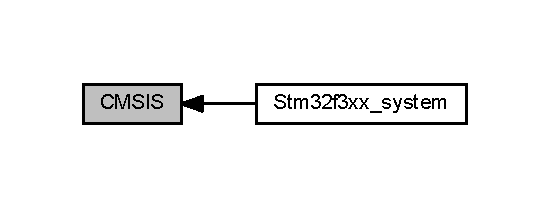
\includegraphics[width=264pt]{group___c_m_s_i_s}
\end{center}
\end{figure}
\subsection*{Modules}
\begin{DoxyCompactItemize}
\item 
\hyperlink{group__stm32f3xx__system}{Stm32f3xx\+\_\+system}
\end{DoxyCompactItemize}


\subsection{Detailed Description}

\hypertarget{group__stm32f3xx__system}{}\section{Stm32f3xx\+\_\+system}
\label{group__stm32f3xx__system}\index{Stm32f3xx\+\_\+system@{Stm32f3xx\+\_\+system}}
Collaboration diagram for Stm32f3xx\+\_\+system\+:\nopagebreak
\begin{figure}[H]
\begin{center}
\leavevmode
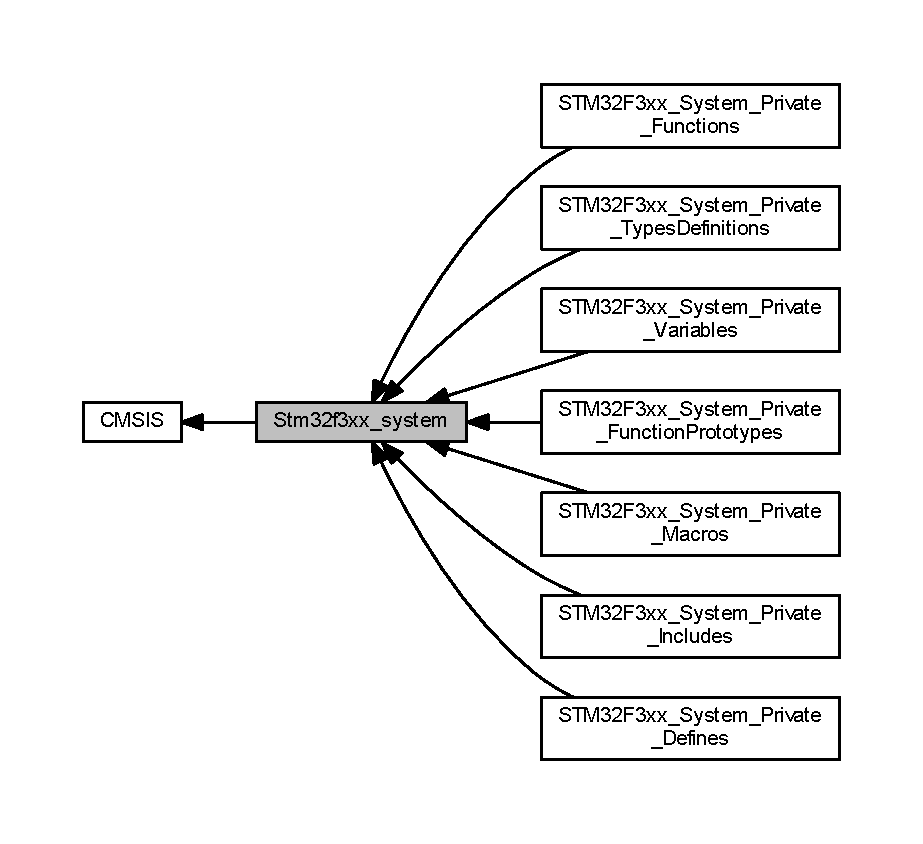
\includegraphics[width=350pt]{group__stm32f3xx__system}
\end{center}
\end{figure}
\subsection*{Modules}
\begin{DoxyCompactItemize}
\item 
\hyperlink{group___s_t_m32_f3xx___system___private___includes}{S\+T\+M32\+F3xx\+\_\+\+System\+\_\+\+Private\+\_\+\+Includes}
\item 
\hyperlink{group___s_t_m32_f3xx___system___private___types_definitions}{S\+T\+M32\+F3xx\+\_\+\+System\+\_\+\+Private\+\_\+\+Types\+Definitions}
\item 
\hyperlink{group___s_t_m32_f3xx___system___private___defines}{S\+T\+M32\+F3xx\+\_\+\+System\+\_\+\+Private\+\_\+\+Defines}
\item 
\hyperlink{group___s_t_m32_f3xx___system___private___macros}{S\+T\+M32\+F3xx\+\_\+\+System\+\_\+\+Private\+\_\+\+Macros}
\item 
\hyperlink{group___s_t_m32_f3xx___system___private___variables}{S\+T\+M32\+F3xx\+\_\+\+System\+\_\+\+Private\+\_\+\+Variables}
\item 
\hyperlink{group___s_t_m32_f3xx___system___private___function_prototypes}{S\+T\+M32\+F3xx\+\_\+\+System\+\_\+\+Private\+\_\+\+Function\+Prototypes}
\item 
\hyperlink{group___s_t_m32_f3xx___system___private___functions}{S\+T\+M32\+F3xx\+\_\+\+System\+\_\+\+Private\+\_\+\+Functions}
\end{DoxyCompactItemize}


\subsection{Detailed Description}

\hypertarget{group___s_t_m32_f3xx___system___private___includes}{}\section{S\+T\+M32\+F3xx\+\_\+\+System\+\_\+\+Private\+\_\+\+Includes}
\label{group___s_t_m32_f3xx___system___private___includes}\index{S\+T\+M32\+F3xx\+\_\+\+System\+\_\+\+Private\+\_\+\+Includes@{S\+T\+M32\+F3xx\+\_\+\+System\+\_\+\+Private\+\_\+\+Includes}}
Collaboration diagram for S\+T\+M32\+F3xx\+\_\+\+System\+\_\+\+Private\+\_\+\+Includes\+:\nopagebreak
\begin{figure}[H]
\begin{center}
\leavevmode
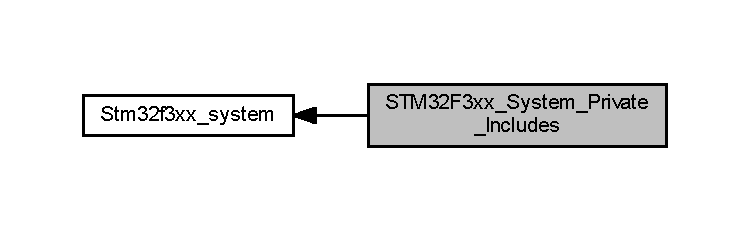
\includegraphics[width=350pt]{group___s_t_m32_f3xx___system___private___includes}
\end{center}
\end{figure}

\hypertarget{group___s_t_m32_f3xx___system___private___types_definitions}{}\section{S\+T\+M32\+F3xx\+\_\+\+System\+\_\+\+Private\+\_\+\+Types\+Definitions}
\label{group___s_t_m32_f3xx___system___private___types_definitions}\index{S\+T\+M32\+F3xx\+\_\+\+System\+\_\+\+Private\+\_\+\+Types\+Definitions@{S\+T\+M32\+F3xx\+\_\+\+System\+\_\+\+Private\+\_\+\+Types\+Definitions}}
Collaboration diagram for S\+T\+M32\+F3xx\+\_\+\+System\+\_\+\+Private\+\_\+\+Types\+Definitions\+:\nopagebreak
\begin{figure}[H]
\begin{center}
\leavevmode
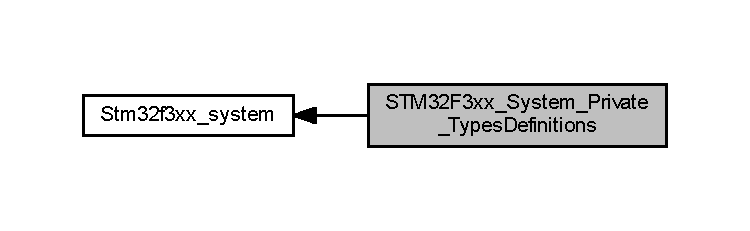
\includegraphics[width=350pt]{group___s_t_m32_f3xx___system___private___types_definitions}
\end{center}
\end{figure}

\hypertarget{group___s_t_m32_f3xx___system___private___defines}{}\section{S\+T\+M32\+F3xx\+\_\+\+System\+\_\+\+Private\+\_\+\+Defines}
\label{group___s_t_m32_f3xx___system___private___defines}\index{S\+T\+M32\+F3xx\+\_\+\+System\+\_\+\+Private\+\_\+\+Defines@{S\+T\+M32\+F3xx\+\_\+\+System\+\_\+\+Private\+\_\+\+Defines}}
Collaboration diagram for S\+T\+M32\+F3xx\+\_\+\+System\+\_\+\+Private\+\_\+\+Defines\+:\nopagebreak
\begin{figure}[H]
\begin{center}
\leavevmode
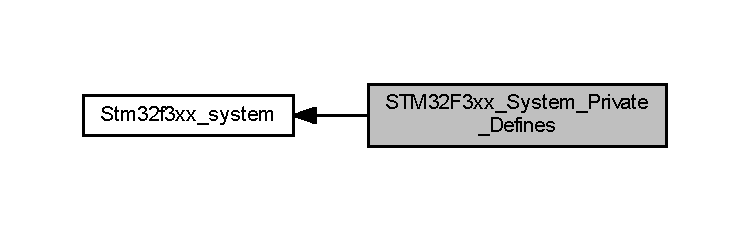
\includegraphics[width=350pt]{group___s_t_m32_f3xx___system___private___defines}
\end{center}
\end{figure}
\subsection*{Macros}
\begin{DoxyCompactItemize}
\item 
\#define \hyperlink{group___s_t_m32_f3xx___system___private___defines_gaeafcff4f57440c60e64812dddd13e7cb}{H\+S\+E\+\_\+\+V\+A\+L\+U\+E}~((uint32\+\_\+t)8000000)
\item 
\#define \hyperlink{group___s_t_m32_f3xx___system___private___defines_gaaa8c76e274d0f6dd2cefb5d0b17fbc37}{H\+S\+I\+\_\+\+V\+A\+L\+U\+E}~((uint32\+\_\+t)8000000)
\item 
\#define \hyperlink{group___s_t_m32_f3xx___system___private___defines_ga40e1495541cbb4acbe3f1819bd87a9fe}{V\+E\+C\+T\+\_\+\+T\+A\+B\+\_\+\+O\+F\+F\+S\+E\+T}~0x0
\end{DoxyCompactItemize}


\subsection{Detailed Description}


\subsection{Macro Definition Documentation}
\hypertarget{group___s_t_m32_f3xx___system___private___defines_gaeafcff4f57440c60e64812dddd13e7cb}{}\index{S\+T\+M32\+F3xx\+\_\+\+System\+\_\+\+Private\+\_\+\+Defines@{S\+T\+M32\+F3xx\+\_\+\+System\+\_\+\+Private\+\_\+\+Defines}!H\+S\+E\+\_\+\+V\+A\+L\+U\+E@{H\+S\+E\+\_\+\+V\+A\+L\+U\+E}}
\index{H\+S\+E\+\_\+\+V\+A\+L\+U\+E@{H\+S\+E\+\_\+\+V\+A\+L\+U\+E}!S\+T\+M32\+F3xx\+\_\+\+System\+\_\+\+Private\+\_\+\+Defines@{S\+T\+M32\+F3xx\+\_\+\+System\+\_\+\+Private\+\_\+\+Defines}}
\subsubsection[{H\+S\+E\+\_\+\+V\+A\+L\+U\+E}]{\setlength{\rightskip}{0pt plus 5cm}\#define H\+S\+E\+\_\+\+V\+A\+L\+U\+E~((uint32\+\_\+t)8000000)}\label{group___s_t_m32_f3xx___system___private___defines_gaeafcff4f57440c60e64812dddd13e7cb}
Default value of the External oscillator in Hz. This value can be provided and adapted by the user application. \hypertarget{group___s_t_m32_f3xx___system___private___defines_gaaa8c76e274d0f6dd2cefb5d0b17fbc37}{}\index{S\+T\+M32\+F3xx\+\_\+\+System\+\_\+\+Private\+\_\+\+Defines@{S\+T\+M32\+F3xx\+\_\+\+System\+\_\+\+Private\+\_\+\+Defines}!H\+S\+I\+\_\+\+V\+A\+L\+U\+E@{H\+S\+I\+\_\+\+V\+A\+L\+U\+E}}
\index{H\+S\+I\+\_\+\+V\+A\+L\+U\+E@{H\+S\+I\+\_\+\+V\+A\+L\+U\+E}!S\+T\+M32\+F3xx\+\_\+\+System\+\_\+\+Private\+\_\+\+Defines@{S\+T\+M32\+F3xx\+\_\+\+System\+\_\+\+Private\+\_\+\+Defines}}
\subsubsection[{H\+S\+I\+\_\+\+V\+A\+L\+U\+E}]{\setlength{\rightskip}{0pt plus 5cm}\#define H\+S\+I\+\_\+\+V\+A\+L\+U\+E~((uint32\+\_\+t)8000000)}\label{group___s_t_m32_f3xx___system___private___defines_gaaa8c76e274d0f6dd2cefb5d0b17fbc37}
Default value of the Internal oscillator in Hz. This value can be provided and adapted by the user application. \hypertarget{group___s_t_m32_f3xx___system___private___defines_ga40e1495541cbb4acbe3f1819bd87a9fe}{}\index{S\+T\+M32\+F3xx\+\_\+\+System\+\_\+\+Private\+\_\+\+Defines@{S\+T\+M32\+F3xx\+\_\+\+System\+\_\+\+Private\+\_\+\+Defines}!V\+E\+C\+T\+\_\+\+T\+A\+B\+\_\+\+O\+F\+F\+S\+E\+T@{V\+E\+C\+T\+\_\+\+T\+A\+B\+\_\+\+O\+F\+F\+S\+E\+T}}
\index{V\+E\+C\+T\+\_\+\+T\+A\+B\+\_\+\+O\+F\+F\+S\+E\+T@{V\+E\+C\+T\+\_\+\+T\+A\+B\+\_\+\+O\+F\+F\+S\+E\+T}!S\+T\+M32\+F3xx\+\_\+\+System\+\_\+\+Private\+\_\+\+Defines@{S\+T\+M32\+F3xx\+\_\+\+System\+\_\+\+Private\+\_\+\+Defines}}
\subsubsection[{V\+E\+C\+T\+\_\+\+T\+A\+B\+\_\+\+O\+F\+F\+S\+E\+T}]{\setlength{\rightskip}{0pt plus 5cm}\#define V\+E\+C\+T\+\_\+\+T\+A\+B\+\_\+\+O\+F\+F\+S\+E\+T~0x0}\label{group___s_t_m32_f3xx___system___private___defines_ga40e1495541cbb4acbe3f1819bd87a9fe}
$<$ Uncomment the following line if you need to relocate your vector Table in Internal S\+R\+A\+M. Vector Table base offset field. This value must be a multiple of 0x200. 
\hypertarget{group___s_t_m32_f3xx___system___private___macros}{}\section{S\+T\+M32\+F3xx\+\_\+\+System\+\_\+\+Private\+\_\+\+Macros}
\label{group___s_t_m32_f3xx___system___private___macros}\index{S\+T\+M32\+F3xx\+\_\+\+System\+\_\+\+Private\+\_\+\+Macros@{S\+T\+M32\+F3xx\+\_\+\+System\+\_\+\+Private\+\_\+\+Macros}}
Collaboration diagram for S\+T\+M32\+F3xx\+\_\+\+System\+\_\+\+Private\+\_\+\+Macros\+:\nopagebreak
\begin{figure}[H]
\begin{center}
\leavevmode
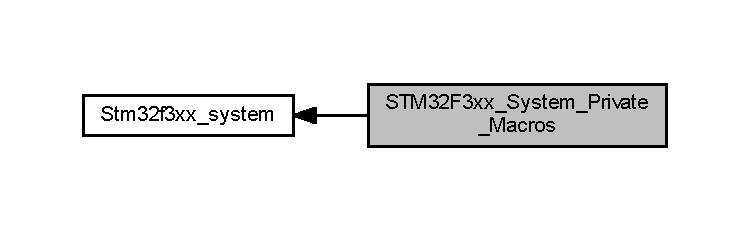
\includegraphics[width=350pt]{group___s_t_m32_f3xx___system___private___macros}
\end{center}
\end{figure}

\hypertarget{group___s_t_m32_f3xx___system___private___variables}{}\section{S\+T\+M32\+F3xx\+\_\+\+System\+\_\+\+Private\+\_\+\+Variables}
\label{group___s_t_m32_f3xx___system___private___variables}\index{S\+T\+M32\+F3xx\+\_\+\+System\+\_\+\+Private\+\_\+\+Variables@{S\+T\+M32\+F3xx\+\_\+\+System\+\_\+\+Private\+\_\+\+Variables}}
Collaboration diagram for S\+T\+M32\+F3xx\+\_\+\+System\+\_\+\+Private\+\_\+\+Variables\+:\nopagebreak
\begin{figure}[H]
\begin{center}
\leavevmode
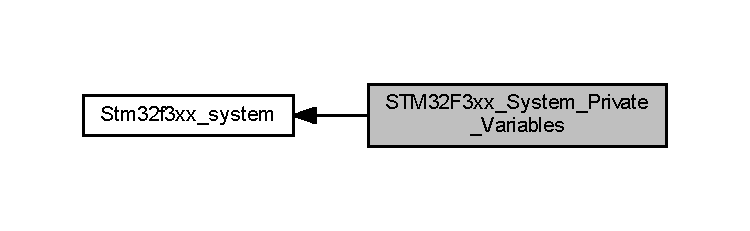
\includegraphics[width=350pt]{group___s_t_m32_f3xx___system___private___variables}
\end{center}
\end{figure}
\subsection*{Variables}
\begin{DoxyCompactItemize}
\item 
\hypertarget{group___s_t_m32_f3xx___system___private___variables_gaa3cd3e43291e81e795d642b79b6088e6}{}uint32\+\_\+t {\bfseries System\+Core\+Clock} = 8000000\label{group___s_t_m32_f3xx___system___private___variables_gaa3cd3e43291e81e795d642b79b6088e6}

\item 
\hypertarget{group___s_t_m32_f3xx___system___private___variables_ga6f9c3580a063d25bfc3acae1db341b12}{}\+\_\+\+\_\+\+I\+O const uint8\+\_\+t {\bfseries A\+H\+B\+Presc\+Table} \mbox{[}16\mbox{]} = \{0, 0, 0, 0, 0, 0, 0, 0, 1, 2, 3, 4, 6, 7, 8, 9\}\label{group___s_t_m32_f3xx___system___private___variables_ga6f9c3580a063d25bfc3acae1db341b12}

\end{DoxyCompactItemize}


\subsection{Detailed Description}

\hypertarget{group___s_t_m32_f3xx___system___private___function_prototypes}{}\section{S\+T\+M32\+F3xx\+\_\+\+System\+\_\+\+Private\+\_\+\+Function\+Prototypes}
\label{group___s_t_m32_f3xx___system___private___function_prototypes}\index{S\+T\+M32\+F3xx\+\_\+\+System\+\_\+\+Private\+\_\+\+Function\+Prototypes@{S\+T\+M32\+F3xx\+\_\+\+System\+\_\+\+Private\+\_\+\+Function\+Prototypes}}
Collaboration diagram for S\+T\+M32\+F3xx\+\_\+\+System\+\_\+\+Private\+\_\+\+Function\+Prototypes\+:\nopagebreak
\begin{figure}[H]
\begin{center}
\leavevmode
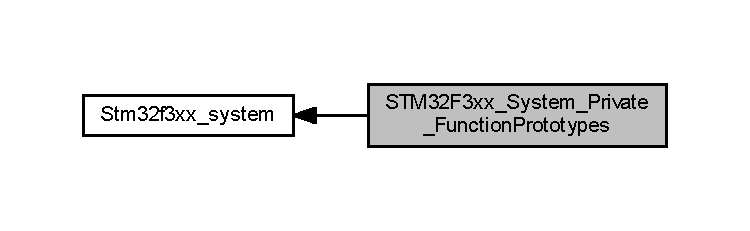
\includegraphics[width=350pt]{group___s_t_m32_f3xx___system___private___function_prototypes}
\end{center}
\end{figure}

\hypertarget{group___s_t_m32_f3xx___system___private___functions}{}\section{S\+T\+M32\+F3xx\+\_\+\+System\+\_\+\+Private\+\_\+\+Functions}
\label{group___s_t_m32_f3xx___system___private___functions}\index{S\+T\+M32\+F3xx\+\_\+\+System\+\_\+\+Private\+\_\+\+Functions@{S\+T\+M32\+F3xx\+\_\+\+System\+\_\+\+Private\+\_\+\+Functions}}
Collaboration diagram for S\+T\+M32\+F3xx\+\_\+\+System\+\_\+\+Private\+\_\+\+Functions\+:\nopagebreak
\begin{figure}[H]
\begin{center}
\leavevmode
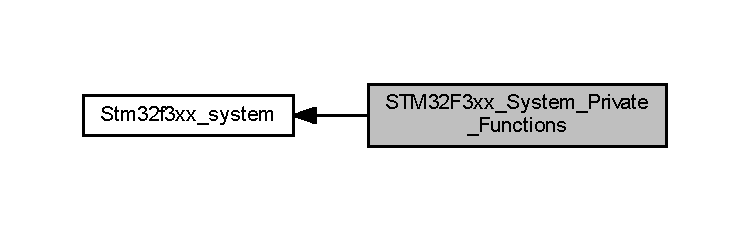
\includegraphics[width=350pt]{group___s_t_m32_f3xx___system___private___functions}
\end{center}
\end{figure}
\subsection*{Functions}
\begin{DoxyCompactItemize}
\item 
void \hyperlink{group___s_t_m32_f3xx___system___private___functions_ga93f514700ccf00d08dbdcff7f1224eb2}{System\+Init} (void)
\begin{DoxyCompactList}\small\item\em Setup the microcontroller system Initialize the F\+P\+U setting, vector table location and the P\+L\+L configuration is reset. \end{DoxyCompactList}\item 
void \hyperlink{group___s_t_m32_f3xx___system___private___functions_gae0c36a9591fe6e9c45ecb21a794f0f0f}{System\+Core\+Clock\+Update} (void)
\begin{DoxyCompactList}\small\item\em Update System\+Core\+Clock variable according to Clock Register Values. The System\+Core\+Clock variable contains the core clock (H\+C\+L\+K), it can be used by the user application to setup the Sys\+Tick timer or configure other parameters. \end{DoxyCompactList}\end{DoxyCompactItemize}


\subsection{Detailed Description}


\subsection{Function Documentation}
\hypertarget{group___s_t_m32_f3xx___system___private___functions_gae0c36a9591fe6e9c45ecb21a794f0f0f}{}\index{S\+T\+M32\+F3xx\+\_\+\+System\+\_\+\+Private\+\_\+\+Functions@{S\+T\+M32\+F3xx\+\_\+\+System\+\_\+\+Private\+\_\+\+Functions}!System\+Core\+Clock\+Update@{System\+Core\+Clock\+Update}}
\index{System\+Core\+Clock\+Update@{System\+Core\+Clock\+Update}!S\+T\+M32\+F3xx\+\_\+\+System\+\_\+\+Private\+\_\+\+Functions@{S\+T\+M32\+F3xx\+\_\+\+System\+\_\+\+Private\+\_\+\+Functions}}
\subsubsection[{System\+Core\+Clock\+Update(void)}]{\setlength{\rightskip}{0pt plus 5cm}void System\+Core\+Clock\+Update (
\begin{DoxyParamCaption}
\item[{void}]{}
\end{DoxyParamCaption}
)}\label{group___s_t_m32_f3xx___system___private___functions_gae0c36a9591fe6e9c45ecb21a794f0f0f}


Update System\+Core\+Clock variable according to Clock Register Values. The System\+Core\+Clock variable contains the core clock (H\+C\+L\+K), it can be used by the user application to setup the Sys\+Tick timer or configure other parameters. 

\begin{DoxyNote}{Note}
Each time the core clock (H\+C\+L\+K) changes, this function must be called to update System\+Core\+Clock variable value. Otherwise, any configuration based on this variable will be incorrect.

-\/ The system frequency computed by this function is not the real frequency in the chip. It is calculated based on the predefined constant and the selected clock source\+:
\end{DoxyNote}

\begin{DoxyItemize}
\item If S\+Y\+S\+C\+L\+K source is H\+S\+I, System\+Core\+Clock will contain the \hyperlink{group___s_t_m32_f3xx___system___private___defines_gaaa8c76e274d0f6dd2cefb5d0b17fbc37}{H\+S\+I\+\_\+\+V\+A\+L\+U\+E($\ast$)}
\item If S\+Y\+S\+C\+L\+K source is H\+S\+E, System\+Core\+Clock will contain the \hyperlink{group___s_t_m32_f3xx___system___private___defines_gaeafcff4f57440c60e64812dddd13e7cb}{H\+S\+E\+\_\+\+V\+A\+L\+U\+E($\ast$$\ast$)}
\item If S\+Y\+S\+C\+L\+K source is P\+L\+L, System\+Core\+Clock will contain the \hyperlink{group___s_t_m32_f3xx___system___private___defines_gaeafcff4f57440c60e64812dddd13e7cb}{H\+S\+E\+\_\+\+V\+A\+L\+U\+E($\ast$$\ast$)} or \hyperlink{group___s_t_m32_f3xx___system___private___defines_gaaa8c76e274d0f6dd2cefb5d0b17fbc37}{H\+S\+I\+\_\+\+V\+A\+L\+U\+E($\ast$)} multiplied/divided by the P\+L\+L factors.
\end{DoxyItemize}

($\ast$) H\+S\+I\+\_\+\+V\+A\+L\+U\+E is a constant defined in stm32f3xx\+\_\+hal.\+h file (default value 8 M\+Hz) but the real value may vary depending on the variations in voltage and temperature.

($\ast$$\ast$) H\+S\+E\+\_\+\+V\+A\+L\+U\+E is a constant defined in stm32f3xx\+\_\+hal.\+h file (default value 8 M\+Hz), user has to ensure that H\+S\+E\+\_\+\+V\+A\+L\+U\+E is same as the real frequency of the crystal used. Otherwise, this function may have wrong result.


\begin{DoxyItemize}
\item The result of this function could be not correct when using fractional value for H\+S\+E crystal.
\end{DoxyItemize}


\begin{DoxyParams}{Parameters}
{\em None} & \\
\hline
\end{DoxyParams}

\begin{DoxyRetVals}{Return values}
{\em None} & \\
\hline
\end{DoxyRetVals}
\hypertarget{group___s_t_m32_f3xx___system___private___functions_ga93f514700ccf00d08dbdcff7f1224eb2}{}\index{S\+T\+M32\+F3xx\+\_\+\+System\+\_\+\+Private\+\_\+\+Functions@{S\+T\+M32\+F3xx\+\_\+\+System\+\_\+\+Private\+\_\+\+Functions}!System\+Init@{System\+Init}}
\index{System\+Init@{System\+Init}!S\+T\+M32\+F3xx\+\_\+\+System\+\_\+\+Private\+\_\+\+Functions@{S\+T\+M32\+F3xx\+\_\+\+System\+\_\+\+Private\+\_\+\+Functions}}
\subsubsection[{System\+Init(void)}]{\setlength{\rightskip}{0pt plus 5cm}void System\+Init (
\begin{DoxyParamCaption}
\item[{void}]{}
\end{DoxyParamCaption}
)}\label{group___s_t_m32_f3xx___system___private___functions_ga93f514700ccf00d08dbdcff7f1224eb2}


Setup the microcontroller system Initialize the F\+P\+U setting, vector table location and the P\+L\+L configuration is reset. 


\begin{DoxyParams}{Parameters}
{\em None} & \\
\hline
\end{DoxyParams}

\begin{DoxyRetVals}{Return values}
{\em None} & \\
\hline
\end{DoxyRetVals}

\chapter{Data Structure Documentation}
\hypertarget{structampelparameter}{}\section{ampelparameter Struct Reference}
\label{structampelparameter}\index{ampelparameter@{ampelparameter}}


{\ttfamily \#include $<$ampel.\+h$>$}

\subsection*{Data Fields}
\begin{DoxyCompactItemize}
\item 
\hypertarget{structampelparameter_ac2f9c5a8ed7b3978c304740db3db8bc4}{}bool {\bfseries modus}\label{structampelparameter_ac2f9c5a8ed7b3978c304740db3db8bc4}

\item 
\hypertarget{structampelparameter_aa3e849a47e5e680b0f4fe0d2d4727126}{}\hyperlink{ampel_8h_a5f4305c91042b570d5d94e83ce6b8012}{ampelzustand} {\bfseries zustand}\label{structampelparameter_aa3e849a47e5e680b0f4fe0d2d4727126}

\item 
\hypertarget{structampelparameter_ad70553c5639d1dbd1db238ba0ede8fc2}{}\hyperlink{ampel_8h_a81b8396a1636de3e1e604ce4935e2f29}{ampelevent} {\bfseries event}\label{structampelparameter_ad70553c5639d1dbd1db238ba0ede8fc2}

\end{DoxyCompactItemize}


\subsection{Detailed Description}
Auflistung der ges. Parameter inkl. Wert zur Bestimmung der Schaltung 

The documentation for this struct was generated from the following file\+:\begin{DoxyCompactItemize}
\item 
src/\hyperlink{ampel_8h}{ampel.\+h}\end{DoxyCompactItemize}

\chapter{File Documentation}
\hypertarget{ampel_8h}{}\section{src/ampel.h File Reference}
\label{ampel_8h}\index{src/ampel.\+h@{src/ampel.\+h}}


Definition der States \& Events.  


{\ttfamily \#include $<$stdbool.\+h$>$}\\*
{\ttfamily \#include $<$stdio.\+h$>$}\\*
{\ttfamily \#include $<$stdlib.\+h$>$}\\*
Include dependency graph for ampel.\+h\+:\nopagebreak
\begin{figure}[H]
\begin{center}
\leavevmode
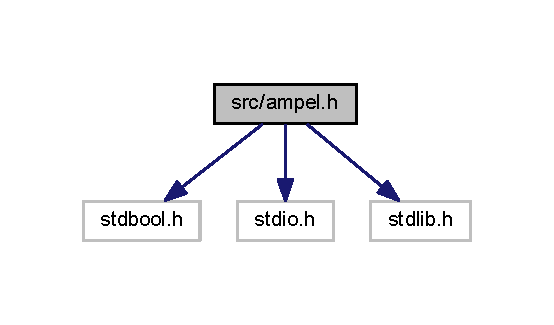
\includegraphics[width=266pt]{ampel_8h__incl}
\end{center}
\end{figure}
This graph shows which files directly or indirectly include this file\+:\nopagebreak
\begin{figure}[H]
\begin{center}
\leavevmode
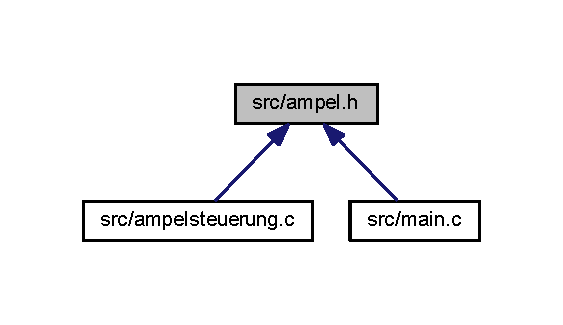
\includegraphics[width=270pt]{ampel_8h__dep__incl}
\end{center}
\end{figure}
\subsection*{Data Structures}
\begin{DoxyCompactItemize}
\item 
struct \hyperlink{structampelparameter}{ampelparameter}
\end{DoxyCompactItemize}
\subsection*{Enumerations}
\begin{DoxyCompactItemize}
\item 
enum \hyperlink{ampel_8h_a5f4305c91042b570d5d94e83ce6b8012}{ampelzustand} \{ \\*
{\bfseries R\+O\+T}, 
{\bfseries R\+O\+T\+\_\+\+G\+E\+L\+B}, 
{\bfseries G\+R\+U\+E\+N}, 
{\bfseries G\+R\+U\+E\+N\+\_\+\+B\+L\+I\+N\+K\+E\+N}, 
\\*
{\bfseries G\+E\+L\+B}, 
{\bfseries G\+E\+L\+B\+\_\+\+B\+L\+I\+N\+K\+E\+N}
 \}
\item 
enum \hyperlink{ampel_8h_a81b8396a1636de3e1e604ce4935e2f29}{ampelevent} \{ \\*
{\bfseries F\+A\+H\+R\+E\+N}, 
{\bfseries H\+A\+L\+T}, 
{\bfseries V\+O\+R\+B\+E\+R\+E\+I\+T\+U\+N\+G\+\_\+\+F\+A\+H\+R\+E\+N}, 
{\bfseries V\+O\+R\+B\+E\+R\+E\+I\+T\+U\+N\+G\+\_\+\+H\+A\+L\+T}, 
\\*
{\bfseries A\+C\+H\+T\+U\+N\+G}, 
{\bfseries F\+A\+L\+S\+E}, 
{\bfseries N\+A\+C\+H\+T\+S\+C\+H\+A\+L\+T\+U\+N\+G\+\_\+\+A\+N}, 
{\bfseries N\+A\+C\+H\+T\+S\+C\+H\+A\+L\+T\+U\+N\+G\+\_\+\+A\+U\+S}
 \}
\end{DoxyCompactItemize}
\subsection*{Functions}
\begin{DoxyCompactItemize}
\item 
\hypertarget{ampel_8h_a591d34377b80002f63ff21438c8b7207}{}void {\bfseries ampel} (\hyperlink{structampelparameter}{ampelparameter} $\ast$ampel)\label{ampel_8h_a591d34377b80002f63ff21438c8b7207}

\end{DoxyCompactItemize}


\subsection{Detailed Description}
Definition der States \& Events. 

\begin{DoxyAuthor}{Author}
Michael Weinberger 
\end{DoxyAuthor}
\begin{DoxyVersion}{Version}
1.\+0 
\end{DoxyVersion}
\begin{DoxyDate}{Date}
20.\+11.\+2015 
\end{DoxyDate}


\subsection{Enumeration Type Documentation}
\hypertarget{ampel_8h_a81b8396a1636de3e1e604ce4935e2f29}{}\index{ampel.\+h@{ampel.\+h}!ampelevent@{ampelevent}}
\index{ampelevent@{ampelevent}!ampel.\+h@{ampel.\+h}}
\subsubsection[{ampelevent}]{\setlength{\rightskip}{0pt plus 5cm}enum {\bf ampelevent}}\label{ampel_8h_a81b8396a1636de3e1e604ce4935e2f29}
Auflistung der Events inklusive Nachtschaltung \hypertarget{ampel_8h_a5f4305c91042b570d5d94e83ce6b8012}{}\index{ampel.\+h@{ampel.\+h}!ampelzustand@{ampelzustand}}
\index{ampelzustand@{ampelzustand}!ampel.\+h@{ampel.\+h}}
\subsubsection[{ampelzustand}]{\setlength{\rightskip}{0pt plus 5cm}enum {\bf ampelzustand}}\label{ampel_8h_a5f4305c91042b570d5d94e83ce6b8012}
Auflistung der Zustaende inklusive der Komponente fuer die Nachtschaltung 
\hypertarget{ampelsteuerung_8c}{}\section{src/ampelsteuerung.c File Reference}
\label{ampelsteuerung_8c}\index{src/ampelsteuerung.\+c@{src/ampelsteuerung.\+c}}


Implementierung einer Event Centric State Machine zur Steuerung einer Ampel.  


{\ttfamily \#include \char`\"{}control.\+h\char`\"{}}\\*
{\ttfamily \#include \char`\"{}ampel.\+h\char`\"{}}\\*
Include dependency graph for ampelsteuerung.\+c\+:\nopagebreak
\begin{figure}[H]
\begin{center}
\leavevmode
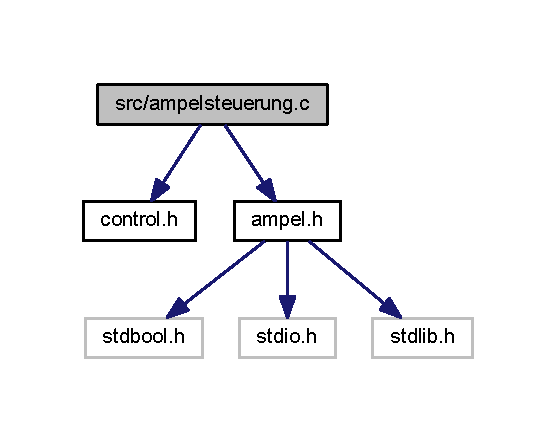
\includegraphics[width=267pt]{ampelsteuerung_8c__incl}
\end{center}
\end{figure}
\subsection*{Functions}
\begin{DoxyCompactItemize}
\item 
void \hyperlink{ampelsteuerung_8c_a8f8d0b2bcdf1febe1191e6bd52015d72}{ampelsteuerung} (\hyperlink{structampelparameter}{ampelparameter} $\ast$repr)
\begin{DoxyCompactList}\small\item\em Implementierung einer Event Centric State Machine zur Steuerung einer Ampel. \end{DoxyCompactList}\end{DoxyCompactItemize}
\subsection*{Variables}
\begin{DoxyCompactItemize}
\item 
\hypertarget{ampelsteuerung_8c_acd2a2ddfbb79edba81215e01a235509a}{}int {\bfseries blink} = 0\label{ampelsteuerung_8c_acd2a2ddfbb79edba81215e01a235509a}

\end{DoxyCompactItemize}


\subsection{Detailed Description}
Implementierung einer Event Centric State Machine zur Steuerung einer Ampel. 

\begin{DoxyAuthor}{Author}
Michael Weinberger 
\end{DoxyAuthor}
\begin{DoxyVersion}{Version}
1.\+0 
\end{DoxyVersion}
\begin{DoxyDate}{Date}
20.\+11.\+2015 
\end{DoxyDate}


\subsection{Function Documentation}
\hypertarget{ampelsteuerung_8c_a8f8d0b2bcdf1febe1191e6bd52015d72}{}\index{ampelsteuerung.\+c@{ampelsteuerung.\+c}!ampelsteuerung@{ampelsteuerung}}
\index{ampelsteuerung@{ampelsteuerung}!ampelsteuerung.\+c@{ampelsteuerung.\+c}}
\subsubsection[{ampelsteuerung(ampelparameter $\ast$repr)}]{\setlength{\rightskip}{0pt plus 5cm}void ampelsteuerung (
\begin{DoxyParamCaption}
\item[{{\bf ampelparameter} $\ast$}]{repr}
\end{DoxyParamCaption}
)}\label{ampelsteuerung_8c_a8f8d0b2bcdf1febe1191e6bd52015d72}


Implementierung einer Event Centric State Machine zur Steuerung einer Ampel. 


\begin{DoxyParams}{Parameters}
{\em none} & \\
\hline
\end{DoxyParams}

\begin{DoxyRetVals}{Return values}
{\em none} & \\
\hline
\end{DoxyRetVals}

\hypertarget{control_8c}{}\section{src/control.c File Reference}
\label{control_8c}\index{src/control.\+c@{src/control.\+c}}


Steuern der benoetigten L\+E\+Ds am Board.  


{\ttfamily \#include \char`\"{}control.\+h\char`\"{}}\\*
{\ttfamily \#include \char`\"{}stm32f3xx.\+h\char`\"{}}\\*
{\ttfamily \#include \char`\"{}stm32f3\+\_\+discovery.\+h\char`\"{}}\\*
Include dependency graph for control.\+c\+:\nopagebreak
\begin{figure}[H]
\begin{center}
\leavevmode
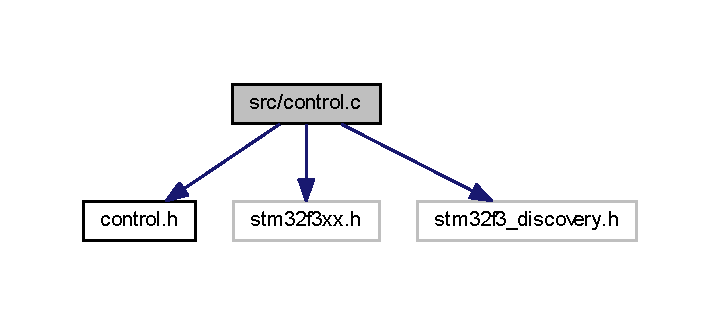
\includegraphics[width=346pt]{control_8c__incl}
\end{center}
\end{figure}
\subsection*{Functions}
\begin{DoxyCompactItemize}
\item 
void \hyperlink{control_8c_a7b3b624857fba1776c75412289a20230}{led\+\_\+init} ()
\begin{DoxyCompactList}\small\item\em Initialisiert die L\+E\+Ds. \end{DoxyCompactList}\item 
void \hyperlink{control_8c_a501391b8794d0beaeaf0dea7a3bdbbb3}{led\+\_\+off} ()
\begin{DoxyCompactList}\small\item\em Schaltet die L\+E\+Ds aus. \end{DoxyCompactList}\item 
void \hyperlink{control_8c_acf33f923d311e918f6ff58d5e36f2820}{led\+\_\+rot} ()
\begin{DoxyCompactList}\small\item\em Die Rot-\/\+Phase der Ampel, 3 Sekunden. \end{DoxyCompactList}\item 
void \hyperlink{control_8c_a7fb6863a7b9298e755f0cdb9344dceff}{led\+\_\+gelb} ()
\begin{DoxyCompactList}\small\item\em Die Gelb-\/\+Phase der Ampel, 1.\+5 Sekunden. \end{DoxyCompactList}\item 
void \hyperlink{control_8c_a0a8db47d447cbe24ac18867af7485301}{led\+\_\+gruen} ()
\begin{DoxyCompactList}\small\item\em Die Gruen-\/\+Phase der Ampel, 3 Sekunden. \end{DoxyCompactList}\item 
void \hyperlink{control_8c_aef77f7543d6efae25faca22475404395}{led\+\_\+rot\+\_\+gelb} ()
\begin{DoxyCompactList}\small\item\em Die Uebergangsphase der Ampel (rot, gelb), 1 Sekunde. \end{DoxyCompactList}\item 
void \hyperlink{control_8c_abac6e28c52d1b1fbf9f3039d0e5fda6d}{led\+\_\+gruen\+\_\+blinken} ()
\begin{DoxyCompactList}\small\item\em 3x gruen blinken, 0.\+5 Sekunden Delay \end{DoxyCompactList}\item 
\hypertarget{control_8c_af6836c9ded67b6022c7d38b45d7e84ac}{}void {\bfseries led\+\_\+gelb\+\_\+blinken} ()\label{control_8c_af6836c9ded67b6022c7d38b45d7e84ac}

\end{DoxyCompactItemize}


\subsection{Detailed Description}
Steuern der benoetigten L\+E\+Ds am Board. 

\begin{DoxyAuthor}{Author}
Michael Weinberger 
\end{DoxyAuthor}
\begin{DoxyVersion}{Version}
1.\+0 
\end{DoxyVersion}
\begin{DoxyDate}{Date}
20.\+11.\+2015 
\end{DoxyDate}


\subsection{Function Documentation}
\hypertarget{control_8c_a7fb6863a7b9298e755f0cdb9344dceff}{}\index{control.\+c@{control.\+c}!led\+\_\+gelb@{led\+\_\+gelb}}
\index{led\+\_\+gelb@{led\+\_\+gelb}!control.\+c@{control.\+c}}
\subsubsection[{led\+\_\+gelb()}]{\setlength{\rightskip}{0pt plus 5cm}void led\+\_\+gelb (
\begin{DoxyParamCaption}
{}
\end{DoxyParamCaption}
)}\label{control_8c_a7fb6863a7b9298e755f0cdb9344dceff}


Die Gelb-\/\+Phase der Ampel, 1.\+5 Sekunden. 


\begin{DoxyParams}{Parameters}
{\em none} & \\
\hline
\end{DoxyParams}

\begin{DoxyRetVals}{Return values}
{\em none} & \\
\hline
\end{DoxyRetVals}
\hypertarget{control_8c_a0a8db47d447cbe24ac18867af7485301}{}\index{control.\+c@{control.\+c}!led\+\_\+gruen@{led\+\_\+gruen}}
\index{led\+\_\+gruen@{led\+\_\+gruen}!control.\+c@{control.\+c}}
\subsubsection[{led\+\_\+gruen()}]{\setlength{\rightskip}{0pt plus 5cm}void led\+\_\+gruen (
\begin{DoxyParamCaption}
{}
\end{DoxyParamCaption}
)}\label{control_8c_a0a8db47d447cbe24ac18867af7485301}


Die Gruen-\/\+Phase der Ampel, 3 Sekunden. 


\begin{DoxyParams}{Parameters}
{\em none} & \\
\hline
\end{DoxyParams}

\begin{DoxyRetVals}{Return values}
{\em none} & \\
\hline
\end{DoxyRetVals}
\hypertarget{control_8c_abac6e28c52d1b1fbf9f3039d0e5fda6d}{}\index{control.\+c@{control.\+c}!led\+\_\+gruen\+\_\+blinken@{led\+\_\+gruen\+\_\+blinken}}
\index{led\+\_\+gruen\+\_\+blinken@{led\+\_\+gruen\+\_\+blinken}!control.\+c@{control.\+c}}
\subsubsection[{led\+\_\+gruen\+\_\+blinken()}]{\setlength{\rightskip}{0pt plus 5cm}void led\+\_\+gruen\+\_\+blinken (
\begin{DoxyParamCaption}
{}
\end{DoxyParamCaption}
)}\label{control_8c_abac6e28c52d1b1fbf9f3039d0e5fda6d}


3x gruen blinken, 0.\+5 Sekunden Delay 


\begin{DoxyParams}{Parameters}
{\em none} & \\
\hline
\end{DoxyParams}

\begin{DoxyRetVals}{Return values}
{\em none} & \\
\hline
\end{DoxyRetVals}
\hypertarget{control_8c_a7b3b624857fba1776c75412289a20230}{}\index{control.\+c@{control.\+c}!led\+\_\+init@{led\+\_\+init}}
\index{led\+\_\+init@{led\+\_\+init}!control.\+c@{control.\+c}}
\subsubsection[{led\+\_\+init()}]{\setlength{\rightskip}{0pt plus 5cm}void led\+\_\+init (
\begin{DoxyParamCaption}
{}
\end{DoxyParamCaption}
)}\label{control_8c_a7b3b624857fba1776c75412289a20230}


Initialisiert die L\+E\+Ds. 


\begin{DoxyParams}{Parameters}
{\em none} & \\
\hline
\end{DoxyParams}

\begin{DoxyRetVals}{Return values}
{\em none} & \\
\hline
\end{DoxyRetVals}
\hypertarget{control_8c_a501391b8794d0beaeaf0dea7a3bdbbb3}{}\index{control.\+c@{control.\+c}!led\+\_\+off@{led\+\_\+off}}
\index{led\+\_\+off@{led\+\_\+off}!control.\+c@{control.\+c}}
\subsubsection[{led\+\_\+off()}]{\setlength{\rightskip}{0pt plus 5cm}void led\+\_\+off (
\begin{DoxyParamCaption}
{}
\end{DoxyParamCaption}
)}\label{control_8c_a501391b8794d0beaeaf0dea7a3bdbbb3}


Schaltet die L\+E\+Ds aus. 


\begin{DoxyParams}{Parameters}
{\em none} & \\
\hline
\end{DoxyParams}

\begin{DoxyRetVals}{Return values}
{\em none} & \\
\hline
\end{DoxyRetVals}
\hypertarget{control_8c_acf33f923d311e918f6ff58d5e36f2820}{}\index{control.\+c@{control.\+c}!led\+\_\+rot@{led\+\_\+rot}}
\index{led\+\_\+rot@{led\+\_\+rot}!control.\+c@{control.\+c}}
\subsubsection[{led\+\_\+rot()}]{\setlength{\rightskip}{0pt plus 5cm}void led\+\_\+rot (
\begin{DoxyParamCaption}
{}
\end{DoxyParamCaption}
)}\label{control_8c_acf33f923d311e918f6ff58d5e36f2820}


Die Rot-\/\+Phase der Ampel, 3 Sekunden. 


\begin{DoxyParams}{Parameters}
{\em none} & \\
\hline
\end{DoxyParams}

\begin{DoxyRetVals}{Return values}
{\em none} & \\
\hline
\end{DoxyRetVals}
\hypertarget{control_8c_aef77f7543d6efae25faca22475404395}{}\index{control.\+c@{control.\+c}!led\+\_\+rot\+\_\+gelb@{led\+\_\+rot\+\_\+gelb}}
\index{led\+\_\+rot\+\_\+gelb@{led\+\_\+rot\+\_\+gelb}!control.\+c@{control.\+c}}
\subsubsection[{led\+\_\+rot\+\_\+gelb()}]{\setlength{\rightskip}{0pt plus 5cm}void led\+\_\+rot\+\_\+gelb (
\begin{DoxyParamCaption}
{}
\end{DoxyParamCaption}
)}\label{control_8c_aef77f7543d6efae25faca22475404395}


Die Uebergangsphase der Ampel (rot, gelb), 1 Sekunde. 


\begin{DoxyParams}{Parameters}
{\em none} & \\
\hline
\end{DoxyParams}

\begin{DoxyRetVals}{Return values}
{\em none} & \\
\hline
\end{DoxyRetVals}

\hypertarget{control_8h}{}\section{src/control.h File Reference}
\label{control_8h}\index{src/control.\+h@{src/control.\+h}}


Definition der Funktionen.  


This graph shows which files directly or indirectly include this file\+:\nopagebreak
\begin{figure}[H]
\begin{center}
\leavevmode
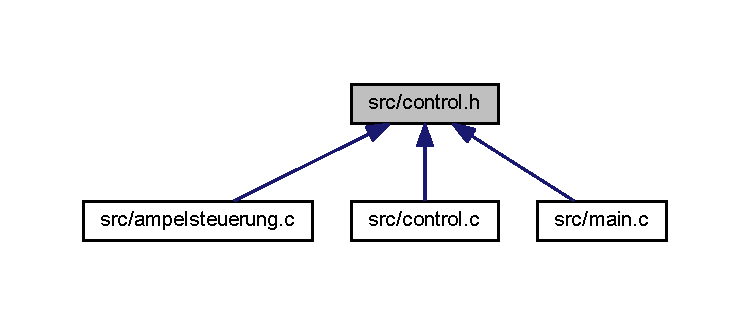
\includegraphics[width=350pt]{control_8h__dep__incl}
\end{center}
\end{figure}
\subsection*{Functions}
\begin{DoxyCompactItemize}
\item 
void \hyperlink{control_8h_acf33f923d311e918f6ff58d5e36f2820}{led\+\_\+rot} ()
\begin{DoxyCompactList}\small\item\em Die Rot-\/\+Phase der Ampel, 3 Sekunden. \end{DoxyCompactList}\item 
void \hyperlink{control_8h_a7fb6863a7b9298e755f0cdb9344dceff}{led\+\_\+gelb} ()
\begin{DoxyCompactList}\small\item\em Die Gelb-\/\+Phase der Ampel, 1.\+5 Sekunden. \end{DoxyCompactList}\item 
void \hyperlink{control_8h_a0a8db47d447cbe24ac18867af7485301}{led\+\_\+gruen} ()
\begin{DoxyCompactList}\small\item\em Die Gruen-\/\+Phase der Ampel, 3 Sekunden. \end{DoxyCompactList}\item 
void \hyperlink{control_8h_aef77f7543d6efae25faca22475404395}{led\+\_\+rot\+\_\+gelb} ()
\begin{DoxyCompactList}\small\item\em Die Uebergangsphase der Ampel (rot, gelb), 1 Sekunde. \end{DoxyCompactList}\item 
void \hyperlink{control_8h_abac6e28c52d1b1fbf9f3039d0e5fda6d}{led\+\_\+gruen\+\_\+blinken} ()
\begin{DoxyCompactList}\small\item\em 3x gruen blinken, 0.\+5 Sekunden Delay \end{DoxyCompactList}\item 
void \hyperlink{control_8h_a7b3b624857fba1776c75412289a20230}{led\+\_\+init} ()
\begin{DoxyCompactList}\small\item\em Initialisiert die L\+E\+Ds. \end{DoxyCompactList}\item 
void \hyperlink{control_8h_a501391b8794d0beaeaf0dea7a3bdbbb3}{led\+\_\+off} ()
\begin{DoxyCompactList}\small\item\em Schaltet die L\+E\+Ds aus. \end{DoxyCompactList}\end{DoxyCompactItemize}


\subsection{Detailed Description}
Definition der Funktionen. 

\begin{DoxyAuthor}{Author}
Michael Weinberger 
\end{DoxyAuthor}
\begin{DoxyVersion}{Version}
1.\+0 
\end{DoxyVersion}
\begin{DoxyDate}{Date}
20.\+11.\+2015 
\end{DoxyDate}


\subsection{Function Documentation}
\hypertarget{control_8h_a7fb6863a7b9298e755f0cdb9344dceff}{}\index{control.\+h@{control.\+h}!led\+\_\+gelb@{led\+\_\+gelb}}
\index{led\+\_\+gelb@{led\+\_\+gelb}!control.\+h@{control.\+h}}
\subsubsection[{led\+\_\+gelb()}]{\setlength{\rightskip}{0pt plus 5cm}void led\+\_\+gelb (
\begin{DoxyParamCaption}
{}
\end{DoxyParamCaption}
)}\label{control_8h_a7fb6863a7b9298e755f0cdb9344dceff}


Die Gelb-\/\+Phase der Ampel, 1.\+5 Sekunden. 


\begin{DoxyParams}{Parameters}
{\em none} & \\
\hline
\end{DoxyParams}

\begin{DoxyRetVals}{Return values}
{\em none} & \\
\hline
\end{DoxyRetVals}
\hypertarget{control_8h_a0a8db47d447cbe24ac18867af7485301}{}\index{control.\+h@{control.\+h}!led\+\_\+gruen@{led\+\_\+gruen}}
\index{led\+\_\+gruen@{led\+\_\+gruen}!control.\+h@{control.\+h}}
\subsubsection[{led\+\_\+gruen()}]{\setlength{\rightskip}{0pt plus 5cm}void led\+\_\+gruen (
\begin{DoxyParamCaption}
{}
\end{DoxyParamCaption}
)}\label{control_8h_a0a8db47d447cbe24ac18867af7485301}


Die Gruen-\/\+Phase der Ampel, 3 Sekunden. 


\begin{DoxyParams}{Parameters}
{\em none} & \\
\hline
\end{DoxyParams}

\begin{DoxyRetVals}{Return values}
{\em none} & \\
\hline
\end{DoxyRetVals}
\hypertarget{control_8h_abac6e28c52d1b1fbf9f3039d0e5fda6d}{}\index{control.\+h@{control.\+h}!led\+\_\+gruen\+\_\+blinken@{led\+\_\+gruen\+\_\+blinken}}
\index{led\+\_\+gruen\+\_\+blinken@{led\+\_\+gruen\+\_\+blinken}!control.\+h@{control.\+h}}
\subsubsection[{led\+\_\+gruen\+\_\+blinken()}]{\setlength{\rightskip}{0pt plus 5cm}void led\+\_\+gruen\+\_\+blinken (
\begin{DoxyParamCaption}
{}
\end{DoxyParamCaption}
)}\label{control_8h_abac6e28c52d1b1fbf9f3039d0e5fda6d}


3x gruen blinken, 0.\+5 Sekunden Delay 


\begin{DoxyParams}{Parameters}
{\em none} & \\
\hline
\end{DoxyParams}

\begin{DoxyRetVals}{Return values}
{\em none} & \\
\hline
\end{DoxyRetVals}
\hypertarget{control_8h_a7b3b624857fba1776c75412289a20230}{}\index{control.\+h@{control.\+h}!led\+\_\+init@{led\+\_\+init}}
\index{led\+\_\+init@{led\+\_\+init}!control.\+h@{control.\+h}}
\subsubsection[{led\+\_\+init()}]{\setlength{\rightskip}{0pt plus 5cm}void led\+\_\+init (
\begin{DoxyParamCaption}
{}
\end{DoxyParamCaption}
)}\label{control_8h_a7b3b624857fba1776c75412289a20230}


Initialisiert die L\+E\+Ds. 


\begin{DoxyParams}{Parameters}
{\em none} & \\
\hline
\end{DoxyParams}

\begin{DoxyRetVals}{Return values}
{\em none} & \\
\hline
\end{DoxyRetVals}
\hypertarget{control_8h_a501391b8794d0beaeaf0dea7a3bdbbb3}{}\index{control.\+h@{control.\+h}!led\+\_\+off@{led\+\_\+off}}
\index{led\+\_\+off@{led\+\_\+off}!control.\+h@{control.\+h}}
\subsubsection[{led\+\_\+off()}]{\setlength{\rightskip}{0pt plus 5cm}void led\+\_\+off (
\begin{DoxyParamCaption}
{}
\end{DoxyParamCaption}
)}\label{control_8h_a501391b8794d0beaeaf0dea7a3bdbbb3}


Schaltet die L\+E\+Ds aus. 


\begin{DoxyParams}{Parameters}
{\em none} & \\
\hline
\end{DoxyParams}

\begin{DoxyRetVals}{Return values}
{\em none} & \\
\hline
\end{DoxyRetVals}
\hypertarget{control_8h_acf33f923d311e918f6ff58d5e36f2820}{}\index{control.\+h@{control.\+h}!led\+\_\+rot@{led\+\_\+rot}}
\index{led\+\_\+rot@{led\+\_\+rot}!control.\+h@{control.\+h}}
\subsubsection[{led\+\_\+rot()}]{\setlength{\rightskip}{0pt plus 5cm}void led\+\_\+rot (
\begin{DoxyParamCaption}
{}
\end{DoxyParamCaption}
)}\label{control_8h_acf33f923d311e918f6ff58d5e36f2820}


Die Rot-\/\+Phase der Ampel, 3 Sekunden. 


\begin{DoxyParams}{Parameters}
{\em none} & \\
\hline
\end{DoxyParams}

\begin{DoxyRetVals}{Return values}
{\em none} & \\
\hline
\end{DoxyRetVals}
\hypertarget{control_8h_aef77f7543d6efae25faca22475404395}{}\index{control.\+h@{control.\+h}!led\+\_\+rot\+\_\+gelb@{led\+\_\+rot\+\_\+gelb}}
\index{led\+\_\+rot\+\_\+gelb@{led\+\_\+rot\+\_\+gelb}!control.\+h@{control.\+h}}
\subsubsection[{led\+\_\+rot\+\_\+gelb()}]{\setlength{\rightskip}{0pt plus 5cm}void led\+\_\+rot\+\_\+gelb (
\begin{DoxyParamCaption}
{}
\end{DoxyParamCaption}
)}\label{control_8h_aef77f7543d6efae25faca22475404395}


Die Uebergangsphase der Ampel (rot, gelb), 1 Sekunde. 


\begin{DoxyParams}{Parameters}
{\em none} & \\
\hline
\end{DoxyParams}

\begin{DoxyRetVals}{Return values}
{\em none} & \\
\hline
\end{DoxyRetVals}

\hypertarget{main_8c}{}\section{src/main.c File Reference}
\label{main_8c}\index{src/main.\+c@{src/main.\+c}}


Hauptklasse.  


{\ttfamily \#include \char`\"{}ampel.\+h\char`\"{}}\\*
{\ttfamily \#include \char`\"{}control.\+h\char`\"{}}\\*
{\ttfamily \#include \char`\"{}stm32f3xx.\+h\char`\"{}}\\*
{\ttfamily \#include \char`\"{}stm32f3\+\_\+discovery.\+h\char`\"{}}\\*
Include dependency graph for main.\+c\+:\nopagebreak
\begin{figure}[H]
\begin{center}
\leavevmode
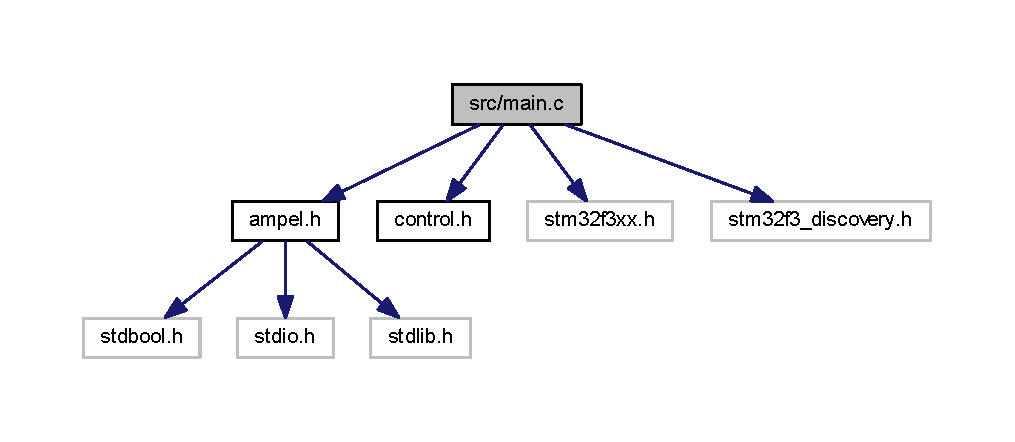
\includegraphics[width=350pt]{main_8c__incl}
\end{center}
\end{figure}
\subsection*{Functions}
\begin{DoxyCompactItemize}
\item 
void \hyperlink{main_8c_a78f3f52a3a37a3930d6f261fff4d00dc}{E\+X\+T\+I0\+\_\+\+Config} ()
\item 
void \hyperlink{main_8c_a807a6ba0d4375cd72bec2b4b01924782}{H\+A\+L\+\_\+\+G\+P\+I\+O\+\_\+\+E\+X\+T\+I\+\_\+\+Callback} (uint16\+\_\+t)
\item 
void \hyperlink{main_8c_a5033855e81ba2071231b60599a3ce9a1}{H\+A\+L\+\_\+\+S\+Y\+S\+T\+I\+C\+K\+\_\+\+Callback} (void)
\item 
\hypertarget{main_8c_a840291bc02cba5474a4cb46a9b9566fe}{}int {\bfseries main} (void)\label{main_8c_a840291bc02cba5474a4cb46a9b9566fe}

\end{DoxyCompactItemize}
\subsection*{Variables}
\begin{DoxyCompactItemize}
\item 
\hypertarget{main_8c_ad2298d5ef1e304cbb6891152a6b8bb90}{}\hyperlink{structampelparameter}{ampelparameter} {\bfseries repr}\label{main_8c_ad2298d5ef1e304cbb6891152a6b8bb90}

\item 
\hypertarget{main_8c_a5e5f27bf68b910793cd70d452ca0deaa}{}\hyperlink{structampelparameter}{ampelparameter} $\ast$ {\bfseries val} = \&repr\label{main_8c_a5e5f27bf68b910793cd70d452ca0deaa}

\end{DoxyCompactItemize}


\subsection{Detailed Description}
Hauptklasse. 

\begin{DoxyAuthor}{Author}
Michael Weinberger 
\end{DoxyAuthor}
\begin{DoxyVersion}{Version}
1.\+0 
\end{DoxyVersion}
\begin{DoxyDate}{Date}
20.\+11.\+2015 
\end{DoxyDate}


\subsection{Function Documentation}
\hypertarget{main_8c_a78f3f52a3a37a3930d6f261fff4d00dc}{}\index{main.\+c@{main.\+c}!E\+X\+T\+I0\+\_\+\+Config@{E\+X\+T\+I0\+\_\+\+Config}}
\index{E\+X\+T\+I0\+\_\+\+Config@{E\+X\+T\+I0\+\_\+\+Config}!main.\+c@{main.\+c}}
\subsubsection[{E\+X\+T\+I0\+\_\+\+Config()}]{\setlength{\rightskip}{0pt plus 5cm}void E\+X\+T\+I0\+\_\+\+Config (
\begin{DoxyParamCaption}
\item[{void}]{}
\end{DoxyParamCaption}
)}\label{main_8c_a78f3f52a3a37a3930d6f261fff4d00dc}
Enablen der Clock, User-\/\+Button konfigurieren, External Interrupt auf Rising Edge Trigger stellen \hypertarget{main_8c_a807a6ba0d4375cd72bec2b4b01924782}{}\index{main.\+c@{main.\+c}!H\+A\+L\+\_\+\+G\+P\+I\+O\+\_\+\+E\+X\+T\+I\+\_\+\+Callback@{H\+A\+L\+\_\+\+G\+P\+I\+O\+\_\+\+E\+X\+T\+I\+\_\+\+Callback}}
\index{H\+A\+L\+\_\+\+G\+P\+I\+O\+\_\+\+E\+X\+T\+I\+\_\+\+Callback@{H\+A\+L\+\_\+\+G\+P\+I\+O\+\_\+\+E\+X\+T\+I\+\_\+\+Callback}!main.\+c@{main.\+c}}
\subsubsection[{H\+A\+L\+\_\+\+G\+P\+I\+O\+\_\+\+E\+X\+T\+I\+\_\+\+Callback(uint16\+\_\+t)}]{\setlength{\rightskip}{0pt plus 5cm}void H\+A\+L\+\_\+\+G\+P\+I\+O\+\_\+\+E\+X\+T\+I\+\_\+\+Callback (
\begin{DoxyParamCaption}
\item[{uint16\+\_\+t}]{G\+P\+I\+O\+\_\+\+Pin}
\end{DoxyParamCaption}
)}\label{main_8c_a807a6ba0d4375cd72bec2b4b01924782}
Der E\+X\+T\+I-\/\+Callback fuer die Ampel \hypertarget{main_8c_a5033855e81ba2071231b60599a3ce9a1}{}\index{main.\+c@{main.\+c}!H\+A\+L\+\_\+\+S\+Y\+S\+T\+I\+C\+K\+\_\+\+Callback@{H\+A\+L\+\_\+\+S\+Y\+S\+T\+I\+C\+K\+\_\+\+Callback}}
\index{H\+A\+L\+\_\+\+S\+Y\+S\+T\+I\+C\+K\+\_\+\+Callback@{H\+A\+L\+\_\+\+S\+Y\+S\+T\+I\+C\+K\+\_\+\+Callback}!main.\+c@{main.\+c}}
\subsubsection[{H\+A\+L\+\_\+\+S\+Y\+S\+T\+I\+C\+K\+\_\+\+Callback(void)}]{\setlength{\rightskip}{0pt plus 5cm}void H\+A\+L\+\_\+\+S\+Y\+S\+T\+I\+C\+K\+\_\+\+Callback (
\begin{DoxyParamCaption}
\item[{void}]{}
\end{DoxyParamCaption}
)}\label{main_8c_a5033855e81ba2071231b60599a3ce9a1}
Der Systick-\/\+Callback fuer die Ampel 
\hypertarget{stm32f3xx__it_8c}{}\section{src/stm32f3xx\+\_\+it.c File Reference}
\label{stm32f3xx__it_8c}\index{src/stm32f3xx\+\_\+it.\+c@{src/stm32f3xx\+\_\+it.\+c}}


Default Interrupt Service Routines.  


{\ttfamily \#include \char`\"{}stm32f3xx\+\_\+hal.\+h\char`\"{}}\\*
{\ttfamily \#include \char`\"{}stm32f3xx.\+h\char`\"{}}\\*
{\ttfamily \#include \char`\"{}stm32f3xx\+\_\+it.\+h\char`\"{}}\\*
{\ttfamily \#include \char`\"{}stm32f3\+\_\+discovery.\+h\char`\"{}}\\*
Include dependency graph for stm32f3xx\+\_\+it.\+c\+:\nopagebreak
\begin{figure}[H]
\begin{center}
\leavevmode
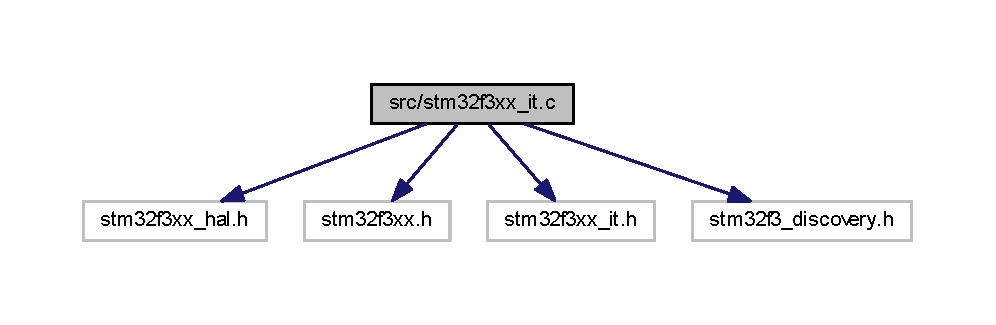
\includegraphics[width=350pt]{stm32f3xx__it_8c__incl}
\end{center}
\end{figure}
\subsection*{Functions}
\begin{DoxyCompactItemize}
\item 
void \hyperlink{stm32f3xx__it_8c_ab5e09814056d617c521549e542639b7e}{Sys\+Tick\+\_\+\+Handler} (void)
\begin{DoxyCompactList}\small\item\em This function handles Sys\+Tick Handler. \end{DoxyCompactList}\item 
\hypertarget{stm32f3xx__it_8c_a17e9789a29a87d2df54f12b94dd1a0b6}{}void {\bfseries E\+X\+T\+I0\+\_\+\+I\+R\+Q\+Handler} (void)\label{stm32f3xx__it_8c_a17e9789a29a87d2df54f12b94dd1a0b6}

\end{DoxyCompactItemize}


\subsection{Detailed Description}
Default Interrupt Service Routines. 

\begin{DoxyAuthor}{Author}
Ac6 
\end{DoxyAuthor}
\begin{DoxyVersion}{Version}
V1.\+0 
\end{DoxyVersion}
\begin{DoxyDate}{Date}
02-\/\+Feb-\/2015 
\end{DoxyDate}


\subsection{Function Documentation}
\hypertarget{stm32f3xx__it_8c_ab5e09814056d617c521549e542639b7e}{}\index{stm32f3xx\+\_\+it.\+c@{stm32f3xx\+\_\+it.\+c}!Sys\+Tick\+\_\+\+Handler@{Sys\+Tick\+\_\+\+Handler}}
\index{Sys\+Tick\+\_\+\+Handler@{Sys\+Tick\+\_\+\+Handler}!stm32f3xx\+\_\+it.\+c@{stm32f3xx\+\_\+it.\+c}}
\subsubsection[{Sys\+Tick\+\_\+\+Handler(void)}]{\setlength{\rightskip}{0pt plus 5cm}void Sys\+Tick\+\_\+\+Handler (
\begin{DoxyParamCaption}
\item[{void}]{}
\end{DoxyParamCaption}
)}\label{stm32f3xx__it_8c_ab5e09814056d617c521549e542639b7e}


This function handles Sys\+Tick Handler. 


\begin{DoxyParams}{Parameters}
{\em None} & \\
\hline
\end{DoxyParams}

\begin{DoxyRetVals}{Return values}
{\em None} & \\
\hline
\end{DoxyRetVals}

\hypertarget{system__stm32f3xx_8c}{}\section{src/system\+\_\+stm32f3xx.c File Reference}
\label{system__stm32f3xx_8c}\index{src/system\+\_\+stm32f3xx.\+c@{src/system\+\_\+stm32f3xx.\+c}}


C\+M\+S\+I\+S Cortex-\/\+M4 Device Peripheral Access Layer System Source File.  


{\ttfamily \#include \char`\"{}stm32f3xx.\+h\char`\"{}}\\*
Include dependency graph for system\+\_\+stm32f3xx.\+c\+:\nopagebreak
\begin{figure}[H]
\begin{center}
\leavevmode
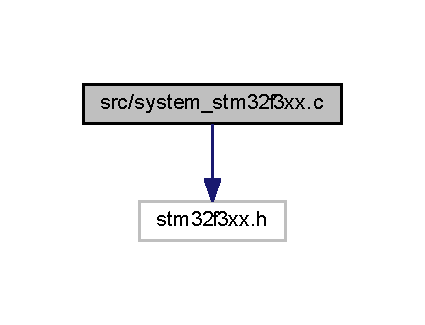
\includegraphics[width=204pt]{system__stm32f3xx_8c__incl}
\end{center}
\end{figure}
\subsection*{Macros}
\begin{DoxyCompactItemize}
\item 
\#define \hyperlink{group___s_t_m32_f3xx___system___private___defines_gaeafcff4f57440c60e64812dddd13e7cb}{H\+S\+E\+\_\+\+V\+A\+L\+U\+E}~((uint32\+\_\+t)8000000)
\item 
\#define \hyperlink{group___s_t_m32_f3xx___system___private___defines_gaaa8c76e274d0f6dd2cefb5d0b17fbc37}{H\+S\+I\+\_\+\+V\+A\+L\+U\+E}~((uint32\+\_\+t)8000000)
\item 
\#define \hyperlink{group___s_t_m32_f3xx___system___private___defines_ga40e1495541cbb4acbe3f1819bd87a9fe}{V\+E\+C\+T\+\_\+\+T\+A\+B\+\_\+\+O\+F\+F\+S\+E\+T}~0x0
\end{DoxyCompactItemize}
\subsection*{Functions}
\begin{DoxyCompactItemize}
\item 
void \hyperlink{group___s_t_m32_f3xx___system___private___functions_ga93f514700ccf00d08dbdcff7f1224eb2}{System\+Init} (void)
\begin{DoxyCompactList}\small\item\em Setup the microcontroller system Initialize the F\+P\+U setting, vector table location and the P\+L\+L configuration is reset. \end{DoxyCompactList}\item 
void \hyperlink{group___s_t_m32_f3xx___system___private___functions_gae0c36a9591fe6e9c45ecb21a794f0f0f}{System\+Core\+Clock\+Update} (void)
\begin{DoxyCompactList}\small\item\em Update System\+Core\+Clock variable according to Clock Register Values. The System\+Core\+Clock variable contains the core clock (H\+C\+L\+K), it can be used by the user application to setup the Sys\+Tick timer or configure other parameters. \end{DoxyCompactList}\end{DoxyCompactItemize}
\subsection*{Variables}
\begin{DoxyCompactItemize}
\item 
\hypertarget{group___s_t_m32_f3xx___system___private___variables_gaa3cd3e43291e81e795d642b79b6088e6}{}uint32\+\_\+t {\bfseries System\+Core\+Clock} = 8000000\label{group___s_t_m32_f3xx___system___private___variables_gaa3cd3e43291e81e795d642b79b6088e6}

\item 
\hypertarget{group___s_t_m32_f3xx___system___private___variables_ga6f9c3580a063d25bfc3acae1db341b12}{}\+\_\+\+\_\+\+I\+O const uint8\+\_\+t {\bfseries A\+H\+B\+Presc\+Table} \mbox{[}16\mbox{]} = \{0, 0, 0, 0, 0, 0, 0, 0, 1, 2, 3, 4, 6, 7, 8, 9\}\label{group___s_t_m32_f3xx___system___private___variables_ga6f9c3580a063d25bfc3acae1db341b12}

\end{DoxyCompactItemize}


\subsection{Detailed Description}
C\+M\+S\+I\+S Cortex-\/\+M4 Device Peripheral Access Layer System Source File. 

\begin{DoxyAuthor}{Author}
M\+C\+D Application Team 
\end{DoxyAuthor}
\begin{DoxyVersion}{Version}
V1.\+2.\+0 
\end{DoxyVersion}
\begin{DoxyDate}{Date}
19-\/\+June-\/2015
\begin{DoxyEnumerate}
\item This file provides two functions and one global variable to be called from user application\+:
\begin{DoxyItemize}
\item \hyperlink{group___s_t_m32_f3xx___system___private___functions_ga93f514700ccf00d08dbdcff7f1224eb2}{System\+Init()}\+: This function is called at startup just after reset and before branch to main program. This call is made inside the \char`\"{}startup\+\_\+stm32f3xx.\+s\char`\"{} file.
\item System\+Core\+Clock variable\+: Contains the core clock (H\+C\+L\+K), it can be used by the user application to setup the Sys\+Tick timer or configure other parameters.
\item \hyperlink{group___s_t_m32_f3xx___system___private___functions_gae0c36a9591fe6e9c45ecb21a794f0f0f}{System\+Core\+Clock\+Update()}\+: Updates the variable System\+Core\+Clock and must be called whenever the core clock is changed during program execution.
\end{DoxyItemize}
\item After each device reset the H\+S\+I (8 M\+Hz) is used as system clock source. Then \hyperlink{group___s_t_m32_f3xx___system___private___functions_ga93f514700ccf00d08dbdcff7f1224eb2}{System\+Init()} function is called, in \char`\"{}startup\+\_\+stm32f3xx.\+s\char`\"{} file, to configure the system clock before to branch to main program.
\end{DoxyEnumerate}
\end{DoxyDate}
\subsection*{3. This file configures the system clock as follows\+: }

\subsubsection*{Supported S\+T\+M32\+F3xx device }

\subsubsection*{System Clock source $\vert$ H\+S\+I }

\subsubsection*{S\+Y\+S\+C\+L\+K(\+Hz) $\vert$ 8000000 }

\subsubsection*{H\+C\+L\+K(\+Hz) $\vert$ 8000000 }

\subsubsection*{A\+H\+B Prescaler $\vert$ 1 }

\subsubsection*{A\+P\+B2 Prescaler $\vert$ 1 }

\subsubsection*{A\+P\+B1 Prescaler $\vert$ 1 }

\subsubsection*{U\+S\+B Clock $\vert$ D\+I\+S\+A\+B\+L\+E }

=============================================================================

\begin{DoxyAttention}{Attention}

\end{DoxyAttention}
\subsubsection*{\begin{center}\copyright{} C\+O\+P\+Y\+R\+I\+G\+H\+T(c) 2015 S\+T\+Microelectronics\end{center} }

Redistribution and use in source and binary forms, with or without modification, are permitted provided that the following conditions are met\+:
\begin{DoxyEnumerate}
\item Redistributions of source code must retain the above copyright notice, this list of conditions and the following disclaimer.
\item Redistributions in binary form must reproduce the above copyright notice, this list of conditions and the following disclaimer in the documentation and/or other materials provided with the distribution.
\item Neither the name of S\+T\+Microelectronics nor the names of its contributors may be used to endorse or promote products derived from this software without specific prior written permission.
\end{DoxyEnumerate}

T\+H\+I\+S S\+O\+F\+T\+W\+A\+R\+E I\+S P\+R\+O\+V\+I\+D\+E\+D B\+Y T\+H\+E C\+O\+P\+Y\+R\+I\+G\+H\+T H\+O\+L\+D\+E\+R\+S A\+N\+D C\+O\+N\+T\+R\+I\+B\+U\+T\+O\+R\+S \char`\"{}\+A\+S I\+S\char`\"{} A\+N\+D A\+N\+Y E\+X\+P\+R\+E\+S\+S O\+R I\+M\+P\+L\+I\+E\+D W\+A\+R\+R\+A\+N\+T\+I\+E\+S, I\+N\+C\+L\+U\+D\+I\+N\+G, B\+U\+T N\+O\+T L\+I\+M\+I\+T\+E\+D T\+O, T\+H\+E I\+M\+P\+L\+I\+E\+D W\+A\+R\+R\+A\+N\+T\+I\+E\+S O\+F M\+E\+R\+C\+H\+A\+N\+T\+A\+B\+I\+L\+I\+T\+Y A\+N\+D F\+I\+T\+N\+E\+S\+S F\+O\+R A P\+A\+R\+T\+I\+C\+U\+L\+A\+R P\+U\+R\+P\+O\+S\+E A\+R\+E D\+I\+S\+C\+L\+A\+I\+M\+E\+D. I\+N N\+O E\+V\+E\+N\+T S\+H\+A\+L\+L T\+H\+E C\+O\+P\+Y\+R\+I\+G\+H\+T H\+O\+L\+D\+E\+R O\+R C\+O\+N\+T\+R\+I\+B\+U\+T\+O\+R\+S B\+E L\+I\+A\+B\+L\+E F\+O\+R A\+N\+Y D\+I\+R\+E\+C\+T, I\+N\+D\+I\+R\+E\+C\+T, I\+N\+C\+I\+D\+E\+N\+T\+A\+L, S\+P\+E\+C\+I\+A\+L, E\+X\+E\+M\+P\+L\+A\+R\+Y, O\+R C\+O\+N\+S\+E\+Q\+U\+E\+N\+T\+I\+A\+L D\+A\+M\+A\+G\+E\+S (I\+N\+C\+L\+U\+D\+I\+N\+G, B\+U\+T N\+O\+T L\+I\+M\+I\+T\+E\+D T\+O, P\+R\+O\+C\+U\+R\+E\+M\+E\+N\+T O\+F S\+U\+B\+S\+T\+I\+T\+U\+T\+E G\+O\+O\+D\+S O\+R S\+E\+R\+V\+I\+C\+E\+S; L\+O\+S\+S O\+F U\+S\+E, D\+A\+T\+A, O\+R P\+R\+O\+F\+I\+T\+S; O\+R B\+U\+S\+I\+N\+E\+S\+S I\+N\+T\+E\+R\+R\+U\+P\+T\+I\+O\+N) H\+O\+W\+E\+V\+E\+R C\+A\+U\+S\+E\+D A\+N\+D O\+N A\+N\+Y T\+H\+E\+O\+R\+Y O\+F L\+I\+A\+B\+I\+L\+I\+T\+Y, W\+H\+E\+T\+H\+E\+R I\+N C\+O\+N\+T\+R\+A\+C\+T, S\+T\+R\+I\+C\+T L\+I\+A\+B\+I\+L\+I\+T\+Y, O\+R T\+O\+R\+T (I\+N\+C\+L\+U\+D\+I\+N\+G N\+E\+G\+L\+I\+G\+E\+N\+C\+E O\+R O\+T\+H\+E\+R\+W\+I\+S\+E) A\+R\+I\+S\+I\+N\+G I\+N A\+N\+Y W\+A\+Y O\+U\+T O\+F T\+H\+E U\+S\+E O\+F T\+H\+I\+S S\+O\+F\+T\+W\+A\+R\+E, E\+V\+E\+N I\+F A\+D\+V\+I\+S\+E\+D O\+F T\+H\+E P\+O\+S\+S\+I\+B\+I\+L\+I\+T\+Y O\+F S\+U\+C\+H D\+A\+M\+A\+G\+E. 
%--- End generated contents ---

% Index
\backmatter
\newpage
\phantomsection
\clearemptydoublepage
\addcontentsline{toc}{chapter}{Index}
\printindex

\end{document}
